%!TEX root = ../cluster_semi.tex
\section{Framework of Ads}
\label{sec:algorithm}
As aforementioned, we propose \name{}, a semi-supervised learning based anomaly detection framework for KPI streams, to tackle the problem of rapid deployment of anomaly detection models for large number of emerging KPI streams, without manual algorithm selection, parameter tuning, or new anomaly labeling for any newly generated KPI streams.
% the challenges introduced by newly generated KPI streams, including algorithm selection, parameter tuning and anomaly labeling.

\begin{figure*}
  \centering
  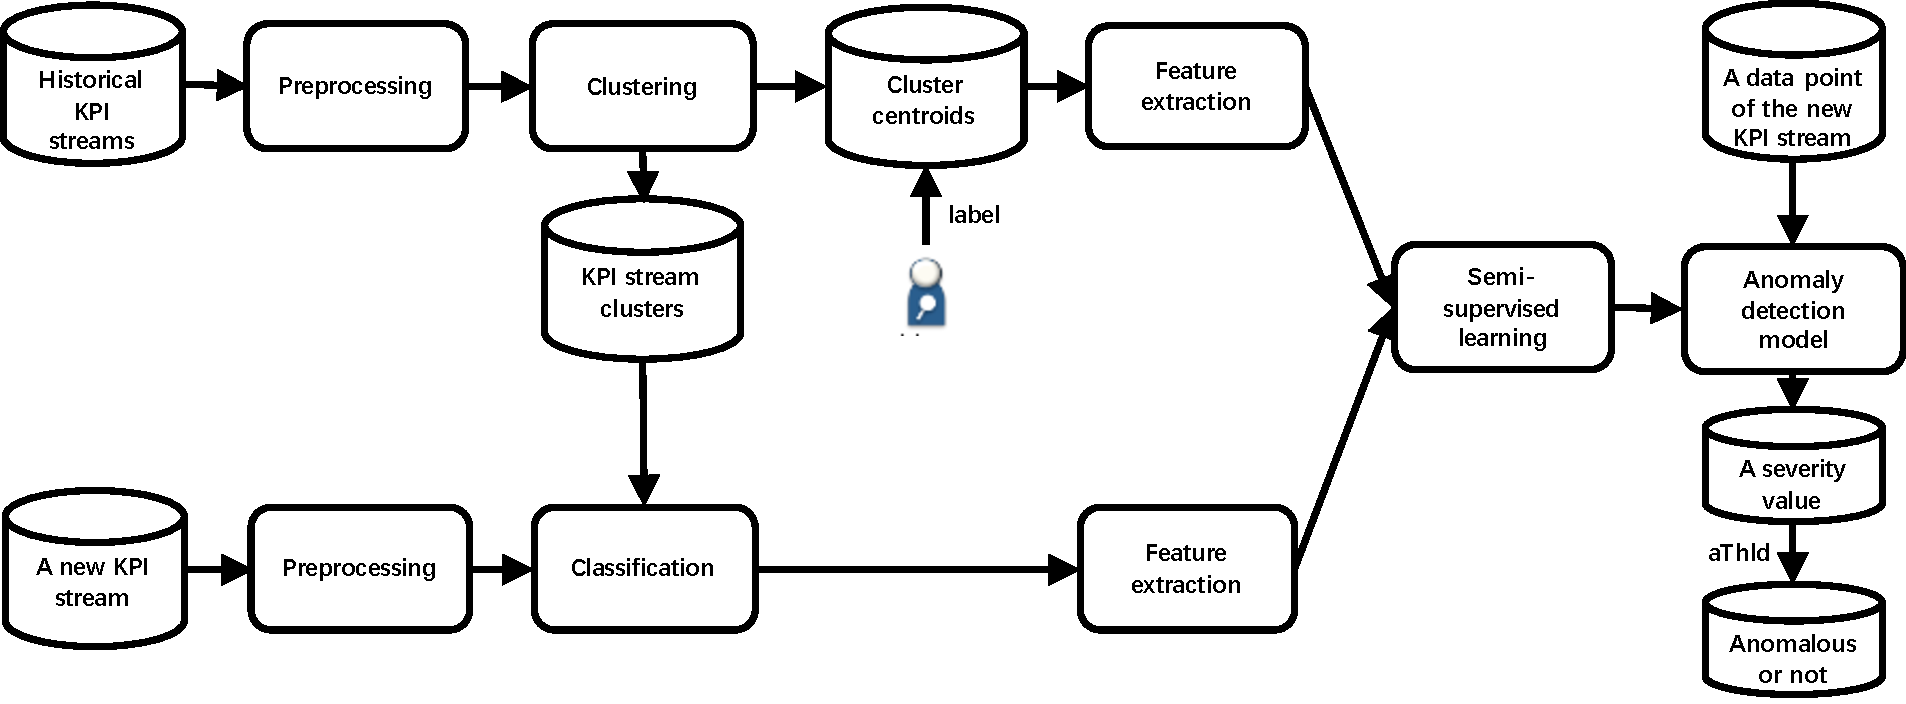
\includegraphics[width=0.9\linewidth]{fig/overview.pdf}
  \caption{
    The framework of~\name{}
  }
  \label{fig:overview}
  \vspace{-6 mm}

\end{figure*}




% Fig.~\ref{fig:overview} give an overview of our algorithm, consists of offline clustering component and online training component. The key techniques are clustering and semi-supervised learning.

Figure~\ref{fig:overview} shows the framework of \name{}.
% \name{} has two main training components: the first component is trained based on historical data, and the second one is trained based on new data.
For historical KPI streams, \name{} preprocesses them with filling missing points and standardization, clusters the preprocessed KPI streams using \ROCKA~(Section~\ref{subsubsec:preprocessing}), and extracts features (namely, output results of different anomaly detection algorithms and parameters) for the KPI streams on cluster centroids (Section~\ref{subsubsec:feature_extraction}).
Similarly, when a new KPI stream is generated, \name~preprocesses it, and classifies it into one of the above clusters (Section~\ref{subsubsec:preprocessing}), after which the features of this new KPI stream are extracted (Section~\ref{subsubsec:feature_extraction}).
Based on the features of the new KPI stream, and the features and labels of the new KPI stream's cluster centroid, 
% Based on the labels and the (anomaly detector) features of the KPI streams on the cluster centroid, and the (anomaly detector) features of the new KPI stream, 
\name~trains a semi-supervised learning model using the CPLE algorithm (Section~\ref{subsubsec:semi_supervised_model}).
% Finally, \name~sets 
Finally, \name~detects anomalies in the new KPI stream based on the above model and the severity threshold (aThld henceforth).
% and the threshold learned from the labeled cluster centroid (Section~\ref{subsubsec:choose_threshold}).


% In offline component, preprocessing is conducted on the historical KPI steams firstly. Next, we group KPI streams into a few clusters, then obtain the centroid of each cluster which represents the shape of a cluster and needs to be labelled. Finally, we calculate anomaly scores by traditional statistical algorithms as features for the data points on these centroids.
% In online component, we proprecess the new KPI stream, assign it to the nearest cluster and extract features. Then we train semi-supervised learning model useing data ponits on labelled centroid and unlabelled new KPI stream to detect anomaly for the future part of this new KPI stream. Finally, we find the appropriate threshold which the point's anomaly score given by model exceeds will be regard as an anomaly.

% After giving an overview of algorithm, we will introduce two components in detail.
% \subsection{Offline Component}
% \label{subsec:offline}

\subsection{Preprocessing and Clustering}
\label{subsubsec:preprocessing}
In Internet-based services, monitoring system malfunctions and/or operator misconfigurations, though occur infrequently, can lead to missing points in KPI streams.
These missing points can bring significant biases to~\name.
Therefore, we fill these missing points using linear interpolation following~\cite{lirobust}. 
% KPI streams can have missing values because of monitoring system malfunctions or human factors, but the percent is usually small. 
% These points can bring biases to our model. So we fill them by linear interpolation simply to eliminate the biases.

In addition, to make KPI steams of different amplitudes and/or length scales comparable, we also standardize KPI streams.
This way, different KPI streams are clustered based on their shapes, rather than the absolute values of amplitudes and/or length scales.

% Another step is standardization. In machine learning, it is widely used to cause algorithms such as gradient descent to take longer to converge. This step is also very important when dealing with KPI streams of different amplitudes and scales~\cite{rakthanmanon2012searching}. Only after standardization, the different KPI streams can be compared and be used for traing semi-supervised learning model together.

% \subsection{Clustering}
% \label{subsubsec:cluster}
% Time series clustering is a challenging and popular issue, which has caught the attention of both research and industrial communities in the past 20 years. Some survey papers~\cite{liao2005clustering, aghabozorgi2015time} summarized large number of published work and common techniques on this topic. Most of these techniques are designed for smooth and idealized data, but in real KPI streams, huge spikes, dips, noises and anomalies can severely change the shape of KPI streams, thus reduce the algorithm's performance. In addition, some of these techniques have high computation complexity~\cite{sakoe1978dynamic}. Another famous method is YADING~\cite{ding2015yading}, but it will take most KPI streams as outliers which mean they are different from each other. 

% We decide to adopt \ROCKA~\cite{lirobust}, a rapid clustering algorithm of KPI streams. It applys moving average to extract baselines that can reduce the biases of noises and anomalies. Additionally, it uses shape-based distance (SBD)~\cite{paparrizos2015k} as distance measure for baselines whose algorithm complexity is reduced to $O(m\log(m))$ by Fast Fourier Transform. Finally it uses DBSCAN~\cite{ester1996density} for clustering and chooses the centroid for every group. The \ROCKA{} algorithm satisfies our real large-scale KPI streams. We simply apply this clustering algorithm and do not improve it.
As discussed in section~\ref{subsec:}, \name~adopts \ROCKA~\cite{lirobust} to group KPI streams into a few clusters, and obtains a centroid KPI stream for each cluster. 
% Note that a
% We simply apply this clustering algorithm and do not improve it. 
% We believe the \ROCKA{} algorithm satisfies our real large-scale KPI streams.

\subsection{Feature Extraction}
\label{subsubsec:feature_extraction}

When training based on historical data, since the KPI stream on the centroid of each cluster represents the cluster's characteristics, we extract the features of the KPI stream on each cluster centroid.
In addition, when training based on new data, we extract the features of the newly generated KPI stream.
The features of the new KPI stream, the features and the anomaly labels of 
the new KPI stream's cluster centroid,
% the KPI stream on the centroid of the cluster to which the new KPI stream belongs, 
together form the training set.

Here we introduce how to extract features for KPI streams.
As is with~\cite{liu2015opprentice}, we use the output results of different anomaly detectors (namely, the anomaly severities measured by anomaly detectors) as the features of KPI streams.
This way, each detector serves as a feature extractor.
% The intuition is that the anomaly severities measured by different anomaly detectors can naturally serve as the features in machine learning, so each detector can serve as a feature extractor

% The centroids represents the common shape of KPI streams in the clusters, they will be a part of the training data in online Component. 
% We need to label anomalies and extract features for data points on them. 
% We implement 14 widely-used traditional statistical algorithms as mentioned in Opprentice~\cite{liu2015opprentice}. 
% Most algorithms have parameters which also affect the performance, so the Opprentice samples some fixed parameters in the parameter space which combine with their algorithms to produce features. 
% These 14 traditional statistical algorithms are representative and cover most types of curves. We have reason to believe that these features are sufficient and general enough.
% Fig.~\ref{fig:feature_extraction} shows the process of feature extraction.

% A unified model is used to represent different anomaly detectors:
% % \begin{equation}
% % \begin{split}
% % \begin{split}
% $$\text{A data point} \xrightarrow[\text{with parameters}]{\text{an anomaly detector}} \text{severity} \xrightarrow[\text{threshold}]{\text{severity}} \{1,0\}$$
% \end{split}
% \end{split}
% \end{equation}
  When an anomaly detector receives an incoming data point of a KPI stream, it internally produces a non-negative value, called \textit{severity}, to measure how anomalous that data point is. 
  For example, historical average~\cite{lee2012threshold} applies how many times of standard deviations the point is away from the mean as the severity, based on the assumption that the KPI stream data follows Gaussian distribution; Holt-Winters~\cite{yan2012argus} uses a residual error (namely, the absolute difference between the actual value and the forecast value of each data point) to measure the severity. 
  In addition, most anomaly detectors are parameterized and have a set of \textit{internal parameters} (say, historical average has one parameter of window length, and Holt-Winters has three parameters $\{\alpha,\beta, \gamma\}$). 
  As a result, both detectors and their internal parameters decide the severity of a given data point.
  % A severity threshold is then needed to transform a severity value into a binary output (\emph{i.e.,}, an anomaly data point (1) or not (0)) for each anomaly detector.
% Afterwards, an anomaly detector further needs a threshold to
%splits the severity space into two parts,
% translate the severity into a binary output, \emph{i.e.,}, anomaly (1) or not (0).   
% We call this threshold the severity threshold.

% In this work, we apply the severity output by a detector as an anomaly feature, for the reason that it denotes how anomalous a data point is according to this detector.
In this work, for each (parameterized) anomaly detector, \name~samples its parameters to generate one or more ``fixed'' anomaly detectors. This way, an anomaly detector with specific sampled parameters acts as a \textit{feature extractor} as follows:

$$\text{A data point} \xrightarrow[\text{}] {\text{anomaly detector + sampled parameters}} \text{feature}$$

The feature extraction, training, and classification (detection) in \name~are all designed to work with individual data points, not anomaly windows, so that the semi-supervised learning algorithm can have enough data for training. Another benefit of this design choice is that the classifier can detect anomalies fast on each data point.

\begin{table}[htp]
\caption{Detectors and sampled parameters used in \name. Some abbreviations are MA (moving average), EWMA (exponentially weighted MA), TSD (time series decomposition), SVD (singular value decomposition), win(dow), and freq(uency). }
\begin{center}
% \begin{tabular}{|l|l|}
\begin{tabular}{|p{4cm}|p{4cm}|}
  \hline
%   \multirow{2}{*}{KPI}&Interval&Length&Labeling time\\
%    &(minute)&(month)&(minute)\\
Detectors  / \#Configurations&Sampled Parameters\\
\hline
\hline
 Simple threshold~\cite{cloudwatch} / 1&none\\
  \hline
 Diff / 3&last-point, last-day, last-week\\
 \hline
 Simple MA~\cite{Choffnes:2010:CSN:1851182.1851228} / 5 &\multirow{3}{105pt}{win = 10, 20, 30, 40, 50 points}\\
   \cline{1-1}
  Weighted MA~\cite{krishnamurthy2003sketch} / 5& \\
  \cline{1-1}
 MA of diff / 5& \\
 \hline
 EWMA~\cite{krishnamurthy2003sketch} / 5& $\alpha$ = 0.1, 0.3, 0.5, 0.7, 0.9\\
 \hline
 TSD~\cite{chen2013provider} / 1& \multirow{4}{105pt}{win = 1 week} \\
  \cline{1-1}
  TSD MAD / 1& \\
   \cline{1-1}
  Historical average~\cite{lee2012threshold} / 1&\\
  \cline{1-1}
  Historical MAD / 1& \\
 \hline
 Holt-Winters~\cite{yan2012argus} / $4^3=64$&
 $\alpha$, $\beta$, $\gamma$ = 0.2, 0.4, 0.6, 0.8\\
 \hline
 SVD~\cite{Mahimkar:2011:RDM:2079296.2079309} / $5\times3=15$&\#row =10, 20, 30, 40, 50 points, \#column =3, 5, 7\\
 \hline
 % Kalman filter~\cite{soule2005combining}&TBC\\
% \hline
  Wavelet~\cite{barford2002signal} / $3\times3=9$&win = 3, 5 ,7 days,\;\;\; freq = low, mid, high \\
 \hline
  ARIMA~\cite{Zhang:2005:NA:1251086.1251116} / 1&Estimation from data\\
 \hline
  \hline
  \multicolumn{2}{|c|}{In total: 14 detectors / 117 configurations}\\
  \hline

\end{tabular}
\end{center}
\label{tab:detector}
\vspace{-6 mm}
% \vspace{-18pt}
\end{table}

Following~\cite{liu2015opprentice}, we implement 14 widely used anomaly detectors in \name.
All the 14 anomaly detectors and their sample parameters are shown in Table~\ref{tab:detector}.



% \begin{figure}
%       \begin{minipage}[h]{1.0\linewidth}
%       \centering
%       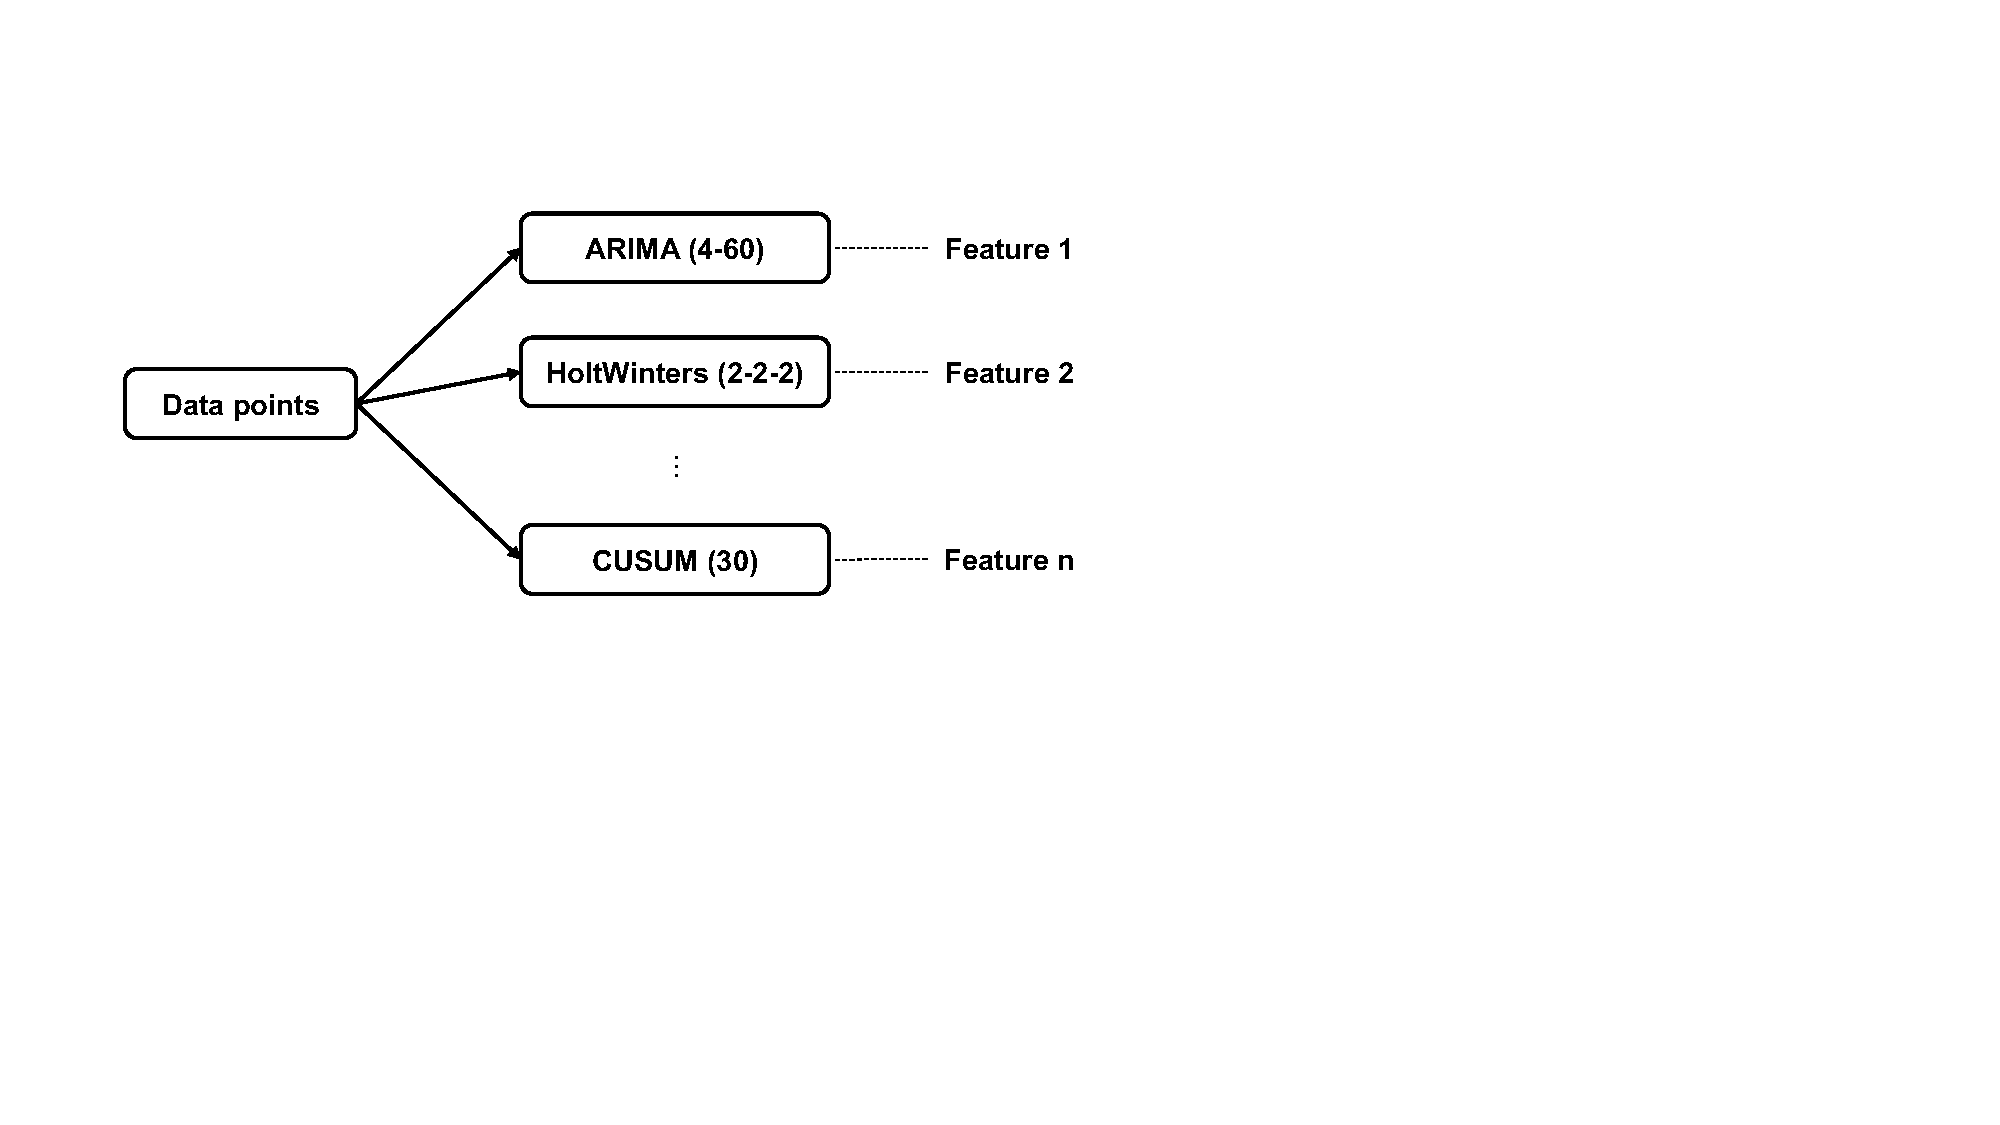
\includegraphics[width=0.9\textwidth]{fig/feature_extraction.pdf}\\
%       \end{minipage}
%       %\vspace{-5 mm}
%       \caption{Feature Extraction.
%       }
%       \label{fig:feature_extraction}
%      % \vspace{-6 mm}
% \end{figure}

% \subsection{Online Component}
% \label{subsec:online}
\subsection{Semi-Supervised Learning}\label{subsubsec:semi_supervised_model}

% After the appearance of a new KPI stream, we do preprocessing, assign it to the nearest cluster according to it's distance to these centroids and extract feature as discussed in~\ref{subsubsec:feature_extraction}. 
% Nextly we train model using data ponits on labelled centroid and unlabelled new KPI stream, then choose threshold.
 
After extracting features of anomaly detectors for both the \emph{labeled} KPI streams on cluster centroids and the \emph{unlabeled} new KPI stream, we try to learn a model which is based on both labeled and unlabeled data, namely a semi-supervised learning model.


As is summarized in~\cite{chapelle2009semi}, different semi-supervised learning models have different advantages and disadvantages.
% Here we briefly discuss common semi-supervised models. 
Among these methods, self-training based methods~\cite{rosenberg2005semi} apply an existing model to ``label'' unlabeled data, and employ the newly labeled data together with the actual labeled data to retrain the model until the prediction result no longer changes or iteration ends.

In this work, we adopt CPLE~\cite{loog2016contrastive}, an extension model of self-training.
CPLE is a resilient semi-supervised learning framework for any supervised learning classifier (base-model henceforth) including random forest, SVM, decision tree, \emph{etc.} 
It takes the prediction probabilities of base-model as input to fully utilize the unlabeled data.
CPLE has the three following advantages: 
\begin{itemize}
  \item  
  CPLE is flexible to change base-model, so we can set its base-model to achieve the best accuracy in anomaly detection. 
  \item CPLE needs low memory complexity, as opposed to graph-based methods~\cite{camps2007semi} which needs $O(n^2)$ memory complexity.
  \item CPLE is more robust than other semi-supervised learning algorithms because it needs no strong assumptions such as (1) the accurate estimation for data distribution of labeled and unlabeled data (as required by  expectation maximization algorithms with generative mixture models~\cite{nigam2000text}) and (2) low density (as required by transductive SVM~\cite{joachims1999transductive}).
  \item CPLE supports incremental learning. 
  Therefore, when more and more data points are added to a KPI stream, we can continuously train \name~to improve its accuracy.
  % As time goes by, there are more and more data points on the KPI stream, and we can continue to train the model to make the detection results more accurate.
\end{itemize}

% Expectation maximization algorithms with generative mixture models~\cite{nigam2000text} strongly assume that all data (with/without labels) comes from the same distribution. 
% % The actual label of unlabeled data can be seen as missing parameters of the distribution. 
% However, the data points of the labeled KPI stream on the cluster centroid and those of the unlabeled new KPI stream (of the same cluster) are not always with the same data distribution because of noises and fluctuations in KPI streams. 
% This will lead to poor performance in accuracy~\cite{cozman2002unlabeled}.
% If clustering based on these noises and fluctuations, too many clusters will be generated to be further used for \name, which is infeasible in practice.

% % If our hypothesis is wrong, the performance of the model will be poor. 
% Transductive SVM~\cite{joachims1999transductive}, a natural extension for SVM, requires low density assumption and can not solve the class-imbalance. 
% Graph-based methods~\cite{camps2007semi} need $O(m^2)$ memory complexity, which causes them not to be applied in large-scale KPI stream set. 



% \begin{figure}
%       \begin{minipage}[h]{1.0\linewidth}
%       \centering
%       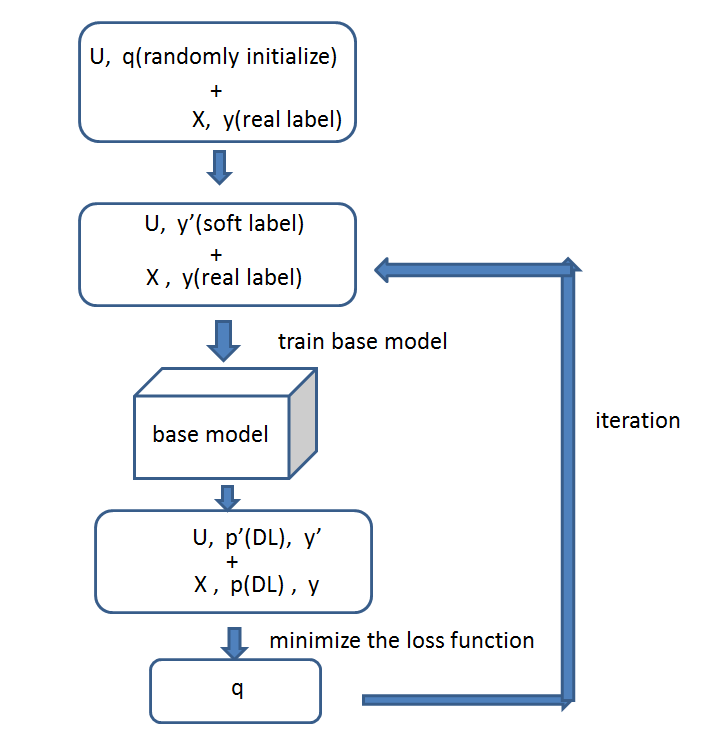
\includegraphics[width=0.9\textwidth]{fig/CPLE.png}\\
%       \end{minipage}
%       %\vspace{-5 mm}
%       \caption{The overview of CPLE.
%       }
%       \label{fig:cple}
%      % \vspace{-6 mm}
% \end{figure}
\name~applies CPLE to detect anomalies for KPI streams as follows.
For a \emph{base-model} (a supervised learning based binary classifier) $f(x)$ with parameter vector $\mathbf{\theta}$, it can be denoted with the form $f(x;\mathbf{\theta})\in\{0,1\}$.
Then the probability that a base-model deems a data point as anomalous is $g(x;\mathbf{\theta})=p(f=1|x,\mathbf{\theta})$, where $g(x;\mathbf{\theta})\in[0,1]$.
In addition, the negative log loss for binary classifiers takes on the general form:
\begin{equation}
\begin{aligned}
J(\mathbf{y,p})&=\log \mathbf{p(y|p)}\\
&=\frac{1}{N}\sum_{i=1}^{N}[y_i\log p_i + (1-y_i)\log (1-p_i)]
\end{aligned}
\label{eqn:log_loss}
\end{equation}
where $N$ is the number of the data points in the KPI streams of training set, $y_i$ is the label of the $i$-th data point and $p_i$ is the $i$-th discriminative likelihood (DL)~\cite{ng2002discriminative}. 
Usually, a machine learning model is aiming to maximize the negative log loss.
% We often maximize the negative log loss to train accurate model.


For the unlabeled data points in the training set (namely, the data points of the newly generated KPI stream), we randomly assign a weight $q_i$ to the $i$-th data point.
The objective of CPLE is to minimize the function
\begin{equation}\label{eq:objective}
E(\mathbf{q,\theta|X,U})=J(\mathbf{y',}g(\mathbf{U;\theta)})-J(\mathbf{y},g(\mathbf{X;\theta}))
\end{equation}
where $\mathbf{X}$ is the data set of labeled data points, $\mathbf{U}$ is the one of unlabeled data points, and $\mathbf{y'}=H(\mathbf{q})$, where
\begin{equation}\label{eq:y}
H({q_i})=\begin{cases}
 1& \text{ if } q_i \geq 0.5\\ 
 0& \text{ if }  q_i < 0.5
\end{cases}
\end{equation}
where $i\in\{1,...,|U|\}$.

This way, (the parameter vector $\theta$ of) the base-model, which serves as the anomaly detection model, is trained based on $(\mathbf{X\cup U})$ using actual and hypothesized labels $(\mathbf{y\cup y'})$, as well as the weights of data points $\mathbf{w}$, where
\begin{equation}\label{eq:weight}
w_i=\begin{cases}
 1& \text{ if } x_i\in \mathbf{X}\\ 
 0&  q_i \text{ otherwise }
\end{cases}
\end{equation}
where $i\in\{1,...,|U|\}$.

In this work, we apply random forest as the base-model of CPLE because of its simplicity, parallelization, and low memory usage, similar to Opprentice~\cite{liu2015opprentice}. We do not claim the adoption of random forest model as our contribution. 



% In CPLE, the unlabeled data can be denoted as $U$ while the labelled data is $X$. Firstly, we randomly initialize $q$ which means soft labels and instance weight for $U$. For each iteration, we minimize the loss function by changing the value of the q:
% \begin{equation}
% q_{semi}=\mathop{\arg\min}_{q}{J_{U}(y',p')-J_{X}(y,p)}
% \label{eqn:cple_loss}
% \end{equation}
% Actually, $q$ is the independent variable of our loss function. The first term of the loss function is calculated on the $U$ while the second is on the $X$. The $y'$ is 1 if $q>0.5$ else 0 and the $y$ is real label. The $p'$ and $p$ can be given by the base-model trained on both $U \cup X$ and hypothesized label $y' \cup y$ with instance weight $q$. The $y'$, $p'$ and $p$ in Eq.~\ref{eqn:cple_loss} are dependent on q. We want to find appropriate q to minimize the loss function.The CPLE is shown in Algorithm~\ref{alg:cple}.


% \begin{algorithm}
%   \caption{CPLE Algorithm}\label{alg:cple}
%   \KwIn{$\mathbf{X}$ : the data set of labeled data points\;
%         $ $ $ $ $ $ $ $ $ $ $ $ $ $ $ $ $ $ $\mathbf{U}$ : the data set of unlabeled data points\;
%         $ $ $ $ $ $ $ $ $ $ $ $ $ $ $ $ $ $ $\mathbf{y}$ : the actual labels of $X$\;
%         $ $ $ $ $ $ $ $ $ $ $ $ $ $ $ $ $ $ $max\_iter$ : the number of maximum iterations\;
%         }
%   \KwOut{$ $ $ $ $ $ $ $ $ $ $ $ $ $ $ $ $ $ $\theta$ : the parameter vector of base-model\;}
%   Randomly initialize $\mathbf{q}$\;
%   \For{each $i\in [0,max\_iter]$}
%     {
%       calculate $\mathbf{y'}$ based on Equation~\ref{eq:y}\;
%       % $y'$ $\gets$ 1 if $q$ $\geq$ 0.5 else 0\;
%       $CPLE$ $model$ $\gets$ base model train on $U \cup X$ and $y' \cup y$ with instance weight $q$\;
%       $p'$ $\gets$ the DL $CPLE$ $model$ gives on $U$\;
%       $p$ $\gets$ the DL $CPLE$ $model$ gives on $X$\;
%       $loss$ $\gets$ ${J_{U}(y',p')-J_{X}(y,p)}$\;
%       $q$ $\gets$ $\mathop{\arg\min} loss$\;
%       \If{loss no longer changes}{
%         break\;
%       }
%     }
  
%   \KwRet{CPLE model}\;
% \end{algorithm}


% From the above we can see that maximizing the negative loss function means pessimistic estimation for unlabeled data. 
% The core idea of CPLE is ``pessimism''. 
% It always assumes the most pessimistic case on unlabeled data, and gives soft labels and instance weight to them to optimize the the worst performance of the algorithm.



 \subsection{Threshold Tuning}
 \label{subsubsec:choose_threshold}
 After obtaining the anomaly detection model (base-model) through semi-supervised learning, \name~computes a non-negative severity value for each data point in the new KPI stream, in order to measure how anomalous this data point is. 
 Then \name{} determines whether a data point is anomalous or not based on a severity threshold (aThld henceforth): if the severity value is larger than aThld, \name{} deems that this data point is anomalous, otherwise, \name{} deems that it is normal.


If we set a default aThld for all KPI streams, \name{} will suffer from low accuracy.
That is because anomalous data points are usually much less than normal ones, and the default threshold usually performs badly in class imbalance settings~\cite{he2008learning}.
%  % because  into which our scenario just falls because .
%  % often have a bad performance in class-imbalance problem().
% % The CPLE can compute anomaly scores meaning certainty for points. 
% % Only if the anomaly score at time $t$ exceeds certain threshold, $x_t$ will be regard as an anomaly. 
% % Therefore, we need to calculate aThld from the training set.
% % We need to choose threshold from the train set rather than using the default one(\EG{}, 0.5) because the 

For a supervised learning based anomaly detection model such as Opprentice~\cite{liu2015opprentice}, it is trained based on a KPI stream, and detects anomalies for \emph{the same KPI stream}.
The severity threshold is calculated based on the \emph{F-score} of the training set.
F-score takes both precision and recall into account. 
It is defined as F-score $=\frac{2*precision*recall}{precision+recall}$. 
The threshold which maximizes the F-score in the training set serves as the threshold.
% % We can use the threshold which maximizes the F-score in train set in the actual scenario.

 As for unsupervised learning based anomaly detection models such as isolation based methods~\cite{ding2013anomaly} and VAE~\cite{xu2018unsupervised}, the KPI streams in the training set have no labels, and thus we cannot calculate any F-score for the training set.
 An \emph{elbow point}~\cite{ketchen1996application} is usually used to set the severity threshold.
 It is the steep part of the cumulative distribution functions (CDFs) curve of severity values.

%  % and we cannot plot PR(Presicion-Recall) curve for them. 
%  % A common method is \emph{elbow point}. A Elbow Point in a curve is the steep part showing significant changes. 
%  % We can plot Cumulative Distribution Function(CDF) for anomaly scores of all train data, and choose the Elbow Point's anomaly score as threshold in the actual scenario.

 To the best of our knowledge, this is the first work using semi-supervised learning model for KPI anomaly detection, which is trained based on a labeled KPI stream and an unlabeled new KPI stream, and detects anomalies for the unlabeled KPI stream.
 Therefore, we try to set aThld based on the F-score of the labeled KPI stream, or the elbow point of the unlabeled one.
 As the empirical experiments described in 
 Section~\ref{subsec:choose_threshold}, setting aThld based on the labeled data performs better than that based on the unlabeled data.
 Therefore, \name{} sets aThld based on the F-score of the labeled KPI stream.
 In other words, aThld is the threshold that maximizes the F-score of the KPI stream on the cluster centroid.




% In \name{}, we use CPLE, a semi-supervised learning model which uses both unlabelled data and labelled data in train set. 
% In ~\ref{subsec:choose_threshold}, We compared the two methos in detail through experiments. Results proves that the threshold given by F-score method on labelled part performace better than Elbow Point on unlabelled part. Actually, with the label information ,F-score method can find the right threshold more precise. Finally, we adopt F-score method in \name{} to choose threhold on the train set and apply it to the actual.




